\section{Executive Summary}

An Agent can be useful for an hour and still fail the work that matters. The
chat ends, the context window is replaced, a different provider takes over, or
the process exits successfully while the actual outcome remains unresolved.
The next Agent then asks the user to reconstruct the project from memory. The
model may be new, but the coordination failure is old: the Work never acquired
an identity independent of the conversation that happened to contain it.

\calloutbox{What Kungfu is}{Kungfu is a local-first product and runtime that
lets a fresh Agent continue the same governed Work without copied chat or a
human restatement. It preserves what is known, what happened, what remains,
which authority applies, and what evidence is required before Work can be
reviewed and completed.}

\subsection{The First Layer}

The complete first-layer product model contains three objects:

\begin{itemize}[leftmargin=*]
  \item a \textbf{Project}: one local directory and its retained Kungfu
  evidence;
  \item \textbf{Work}: one bounded outcome inside that Project; and
  \item an \textbf{Agent}: the selected provider process that performs or
  independently reviews the Work.
\end{itemize}

The ordinary path is equally small:

\begin{quote}
New or Open Project $\rightarrow$ Create or select Work $\rightarrow$ Run
Agent $\rightarrow$ Review and complete Work.
\end{quote}

Users do not need to learn Kungfu's internal ontology before useful work can
begin. Initiative, Assignment, Episode, Assessment, Decision, Warrant, and
Project Cut appear only when evidence, explanation, extension, or review needs
their precision.

\subsection{The First Proof}

Agent Work Lab makes the core promise visible within minutes. Two genuinely
fresh processes work on one bounded Work item. The first stops with a partial
result. The second receives no copied transcript or human explanation,
recovers what was done and what remains, and continues the same Work. A user
can then repeat the experiment with one selected Agent or hand Work to a
different Agent.

The short demonstration is not the full product claim. Its purpose is to let a
new user see the mechanism before relying on it. Deeper value appears when a
real Project survives failed attempts, changed understanding, provider
replacement, restart, and independent review over days.

\begin{center}
\flowbox{Chat ends}
\hfill$\rightarrow$\hfill
\flowbox{Work remains}
\hfill$\rightarrow$\hfill
\flowbox{Fresh Agent continues}
\hfill$\rightarrow$\hfill
\flowbox{Independent review}

\vspace{0.45em}
{\small\color{KFSlate}\textit{The first visible Kungfu product loop.}}
\end{center}

\begin{figure}[htbp]
  \centering
  \begin{evidenceframe}
    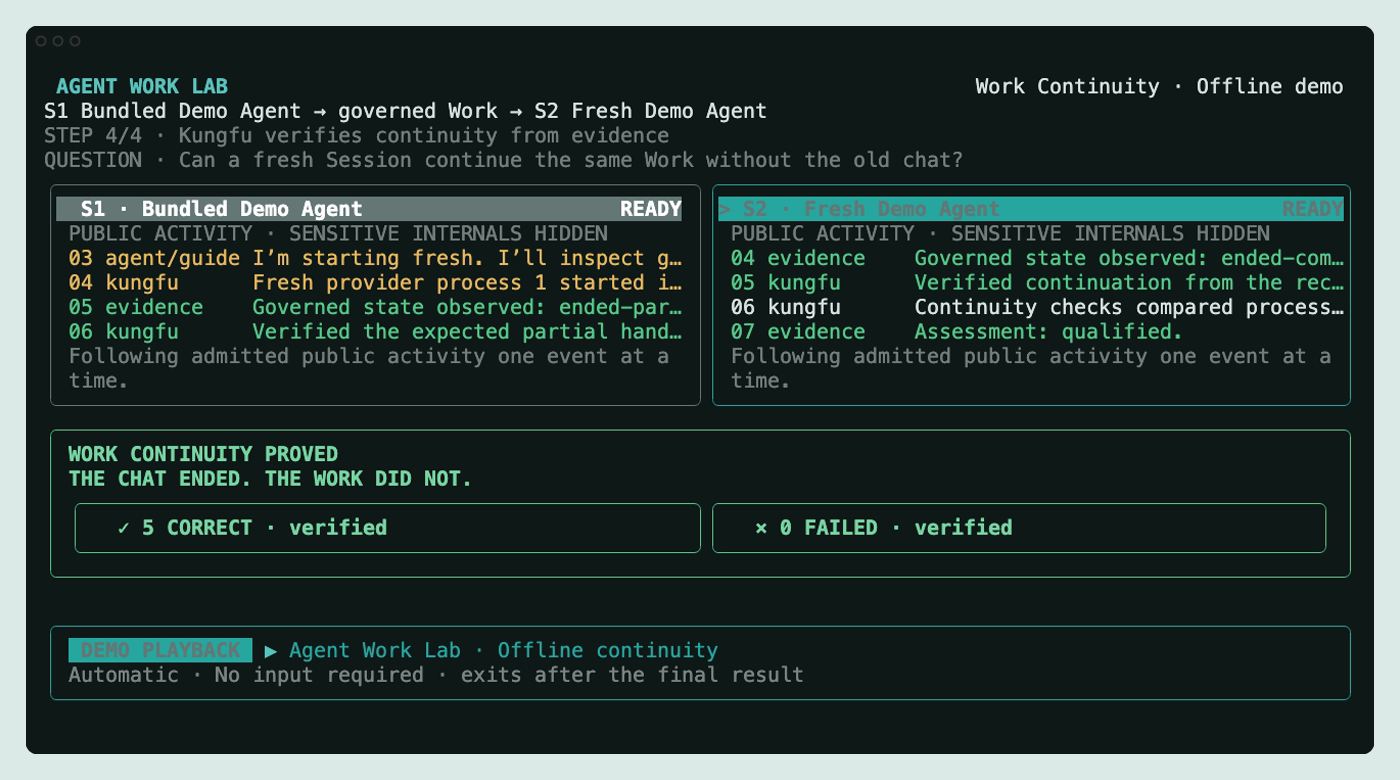
\includegraphics[width=\linewidth]{assets/agent-work-lab-continuity.png}
  \end{evidenceframe}
  \caption{The installed Kungfu Agent Work Lab shows two fresh Sessions
  continuing one governed Work without transcript transfer. The retained
  artifact verifies five bounded continuity checks with zero failures; it does
  not by itself establish longitudinal production continuity.}
  \label{fig:agent-work-lab-continuity}
\end{figure}

\subsection{The Core Argument}

Kungfu is built around four separations:

\begin{itemize}[leftmargin=*]
  \item Work identity is not Agent-process identity.
  \item Admitted fact is not the same thing as observation, claim, or model
  output.
  \item Capability is not authority to act.
  \item A successful process is not an accepted completion decision.
\end{itemize}

These separations are implemented through durable Facts and Episodes,
continuing direction, declared perspective, bounded authority, native Work
responsibility, independent assessment, and content-addressed settlement.
Higher product layers make these mechanisms convenient; they do not acquire
the authority owned by the runtime beneath them.

\subsection{Current Claim Boundary}

Kungfu has source-built product surfaces, mechanically checked first-layer
contracts, and exact installed-artifact evidence for the bounded Agent Work
Lab path. Public Kungfu v4 release artifacts are not yet available. The
current evidence does not establish general production fitness, every provider
or platform, multi-day survival, independent Agent Hub adoption, or a completed
machine-life system. Those boundaries are part of the product record rather
than footnotes to be removed.

This paper explains what Kungfu is now. It ends by identifying a separate
research question opened by the product: if Work identity can survive
replacement of its Agent, can a larger executable subject preserve identity
and direction across replacement of cognition, organs, toolchains, and
machines? That future question belongs to the companion paper on semantic
autopoiesis, not to Kungfu's present product claim.
